% BibTeX
% XeLaTeX

\documentclass{scrarticle}

\usepackage[english]{babel}
\usepackage[natbib,authordate,backend=bibtex]{biblatex-chicago}
   \bibliography{references}
\usepackage[a4paper,top=2cm,bottom=2cm,left=3cm,right=3cm,marginparwidth=1.75cm]{geometry}
\usepackage{wrapfig,graphicx}
   \graphicspath{ {./figures/} }
\usepackage{fontspec}
   \newfontfamily\eva{fairfax_eva_hd.ttf}
\usepackage{xcolor}

\newenvironment{locator}{\tiny\sffamily}

\deffootnote{1.5em}{1em}{\makebox[1.5em][l]{\thefootnotemark}}
   \setlength{\skip\footins}{1.5em} 
   \setlength{\footnotesep}{1em}

\title{Beinecke MS 408}
\date{}

\begin{document}
\maketitle

\section{Introduction}
In the following, mainly to promote easier readability and comparability, a transcription of the manuscript is provided, based on a transliteration by \citet{takahashi_voynich_2004}.
Takahashi's transliteration is obtained in an automatically capitalized version of the \textit{European} or \textit{Extensible Voynich Alphabet} (EVA), using the \textit{Interlinear Transcription Archive Extractor} by \citet{schwerdtfeger_voynich_2004}.\footnote{\citet{schwerdtfeger_voynich_2004} builds on an online archive of Voynich transcriptions that was maintained by Jorge \citet{stolfi_voynich_1998}. For a general overview of transcription efforts, see \citet{zandbergen_text_2023}.}
It is then converted back into glyphs using a font by \citet{bettencourt_voynich_2019}.

Using the manuscript's reproduction in \citet{clemens_voynich_2016}, Takahashi's transliteration is compared with what I am able to make out of the manuscript.
Glyphs that I interpret in another way than Takahashi are printed in \textcolor{orange}{orange}, showing my interpretation.
Removed spaces are marked with \textcolor{orange}{$\frown$} and added spaces are indicated by \textcolor{orange}{$\smile$}.
Especially the recognition of spaces is sometimes very difficult; therefore, my adjustments in this -- just as in any other -- regard should be taken with a certain amount of caution.

Each line of the transcription is preceded by a locator in square brackets, informing the reader about the element a line is part of (i.e., title, paragraph, or label) and assigning the line a number.
For example, a line located at [P2, 9] is part of the page's second paragraph and is the overall ninth line on this page.

For better orientation, a thumbnail of the respective manuscript page is shown in the upper right corner of each transliteration page (scans are taken from ).


\clearpage
\section{Transcription}


%%%%%%
% 1R %
%%%%%%
\subsection{Folio 1, Recto}
\begin{wrapfigure}{r}{0.25\textwidth}
   \centering
   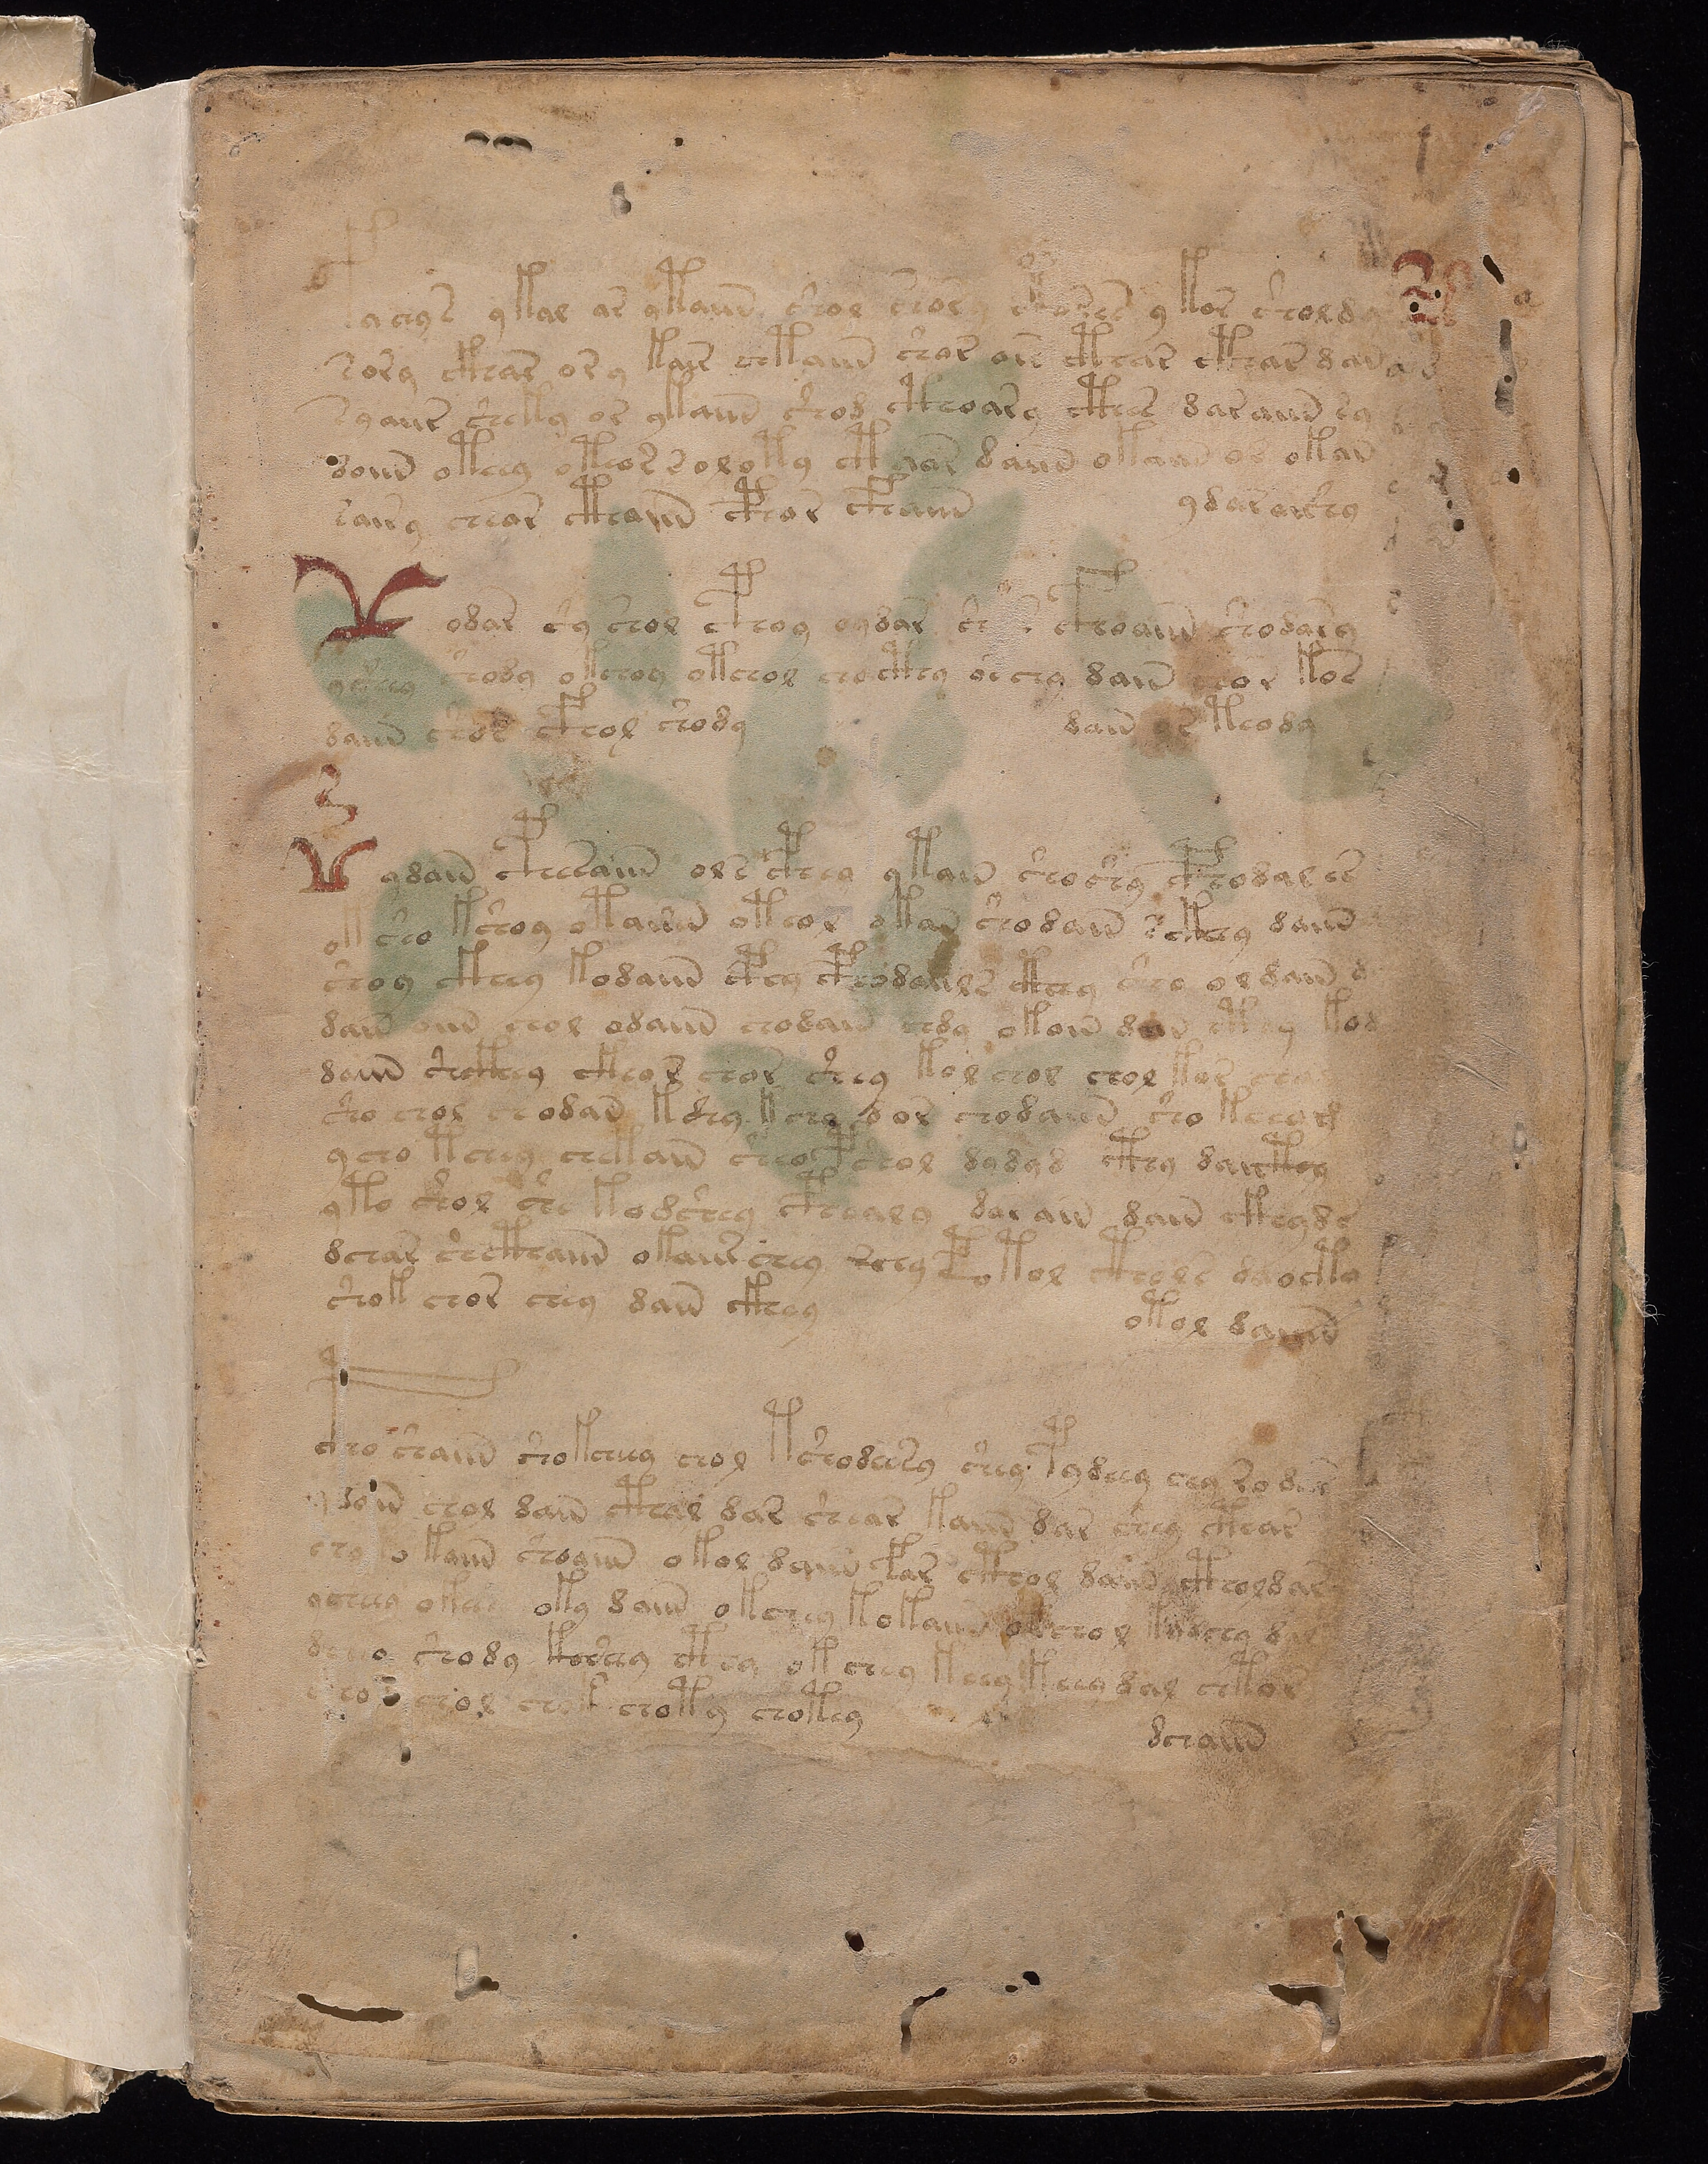
\includegraphics[width=0.25\textwidth]{f1r.jpg}
\end{wrapfigure}

\begin{locator}[P1, 1]\end{locator} {\eva fachys ykal ar ataiin Shol Shory cThres y kor Sholdy}\\
\begin{locator}[P1, 2]\end{locator} {\eva sory cKhar or y kair chtaiin Shar are cThar cThar dan}\\
\begin{locator}[P1, 3]\end{locator} {\eva syaiir Sheky or ykaiin Shod cThoary cThes daraiin s\textcolor{orange}{y}}\\
\begin{locator}[P1, 4]\end{locator} {\eva \textcolor{orange}{d}oiin oteey oteos roloty cTh\textcolor{orange}{i}ar daiin o\textcolor{orange}{k}aiin or okan}\\
\begin{locator}[P1, 5]\end{locator} {\eva dair\textcolor{orange}{$\frown$}y chear cThaiin cPhar cFhaiin}\\
\begin{locator}[T1, 6]\end{locator} {\eva ydaraiShy}\\

\vspace{1em}
\noindent\begin{locator}[P2, 7]\end{locator} {\eva \textcolor{orange}{ü} odar \textcolor{orange}{S$\frown$}y Shol cPhoy oydar Sh*\textcolor{orange}{$\frown$}s cFhoaiin Shodary}\\
\begin{locator}[P2, 8]\end{locator} {\eva yShey Shody okchoy otchol chocThy oschy dain chor kos}\\
\begin{locator}[P2, 9]\end{locator} {\eva daiin Shos cFhol Shody}\\
\begin{locator}[T2, 10]\end{locator} {\eva dain os teody}\\

\vspace{1em}
\noindent\begin{locator}[P3, 11]\end{locator} {\eva \textcolor{orange}{ü} ydain cPhesaiin ol\textcolor{orange}{$\frown$}s cPhey ytain ShoShy cPhodales}\\
\begin{locator}[P3, 12]\end{locator} {\eva okSho kShoy otairin oteol okan Shodain scKhey daiin}\\
\begin{locator}[P3, 13]\end{locator} {\eva Shoy cKhey kodaiin cPhy cPhodaiils cThey She oldain d}\\
\begin{locator}[P3, 14]\end{locator} {\eva dain oiin chol odaiin chodain chdy okain dan cThy kod}\\
\begin{locator}[P3, 15]\end{locator} {\eva daiin ShcKhey \textcolor{orange}{cKh}or chor Shey kol chol chol kor chal}\\
\begin{locator}[P3, 16]\end{locator} {\eva Sho chol Shodan kShy kchy dor chodaiin Sho kchom}\\
\begin{locator}[P3, 17]\end{locator} {\eva ycho tchey ch\textcolor{orange}{e}kain Sheo pShol dydyd cThy daicThy}\\
\begin{locator}[P3, 18]\end{locator} {\eva yto Shol She kodShey cPhealy dasain dain cKhyds}\\
\begin{locator}[P3, 19]\end{locator} {\eva dchar ShcThaiin okaiir\textcolor{orange}{$\frown$}chey rchy potol cThols d\textcolor{orange}{a}octa}\\
\begin{locator}[P3, 20]\end{locator} {\eva Shok chor chey dain cKhey}\\
\begin{locator}[T3, 21]\end{locator} {\eva otol daiiin}\\

\vspace{1em}
\noindent\begin{locator}[P4, 22]\end{locator} {\eva cPho Shaiin Shokcheey chol tShodeesy Shey pydeey chy ro d\textcolor{orange}{ar}}\\
\begin{locator}[P4, 23]\end{locator} {\eva *doin chol dain cThal dar Shear kaiin dar Shey cThar}\\
\begin{locator}[P4, 24]\end{locator} {\eva cho*o kaiin Shoaiin okol daiin far cThol daiin cTholdar}\\
\begin{locator}[P4, 25]\end{locator} {\eva ycheey okay oky daiin okchey kokaiin \textcolor{orange}{of}chol k\textcolor{orange}{ad}chy dal}\\
\begin{locator}[P4, 26]\end{locator} {\eva d\textcolor{orange}{che}o Shody koShey cThy okchey keey keey dal chtor}\\
\begin{locator}[P4, 27]\end{locator} {\eva \textcolor{orange}{ch}o chol chok choty chotey}\\
\begin{locator}[T4, 28]\end{locator} {\eva dchaiin}\\


%%%%%%
% 1V %
%%%%%%
\clearpage
\subsection{Folio 1, Verso}
\begin{wrapfigure}{r}{0.25\textwidth}
   \centering
   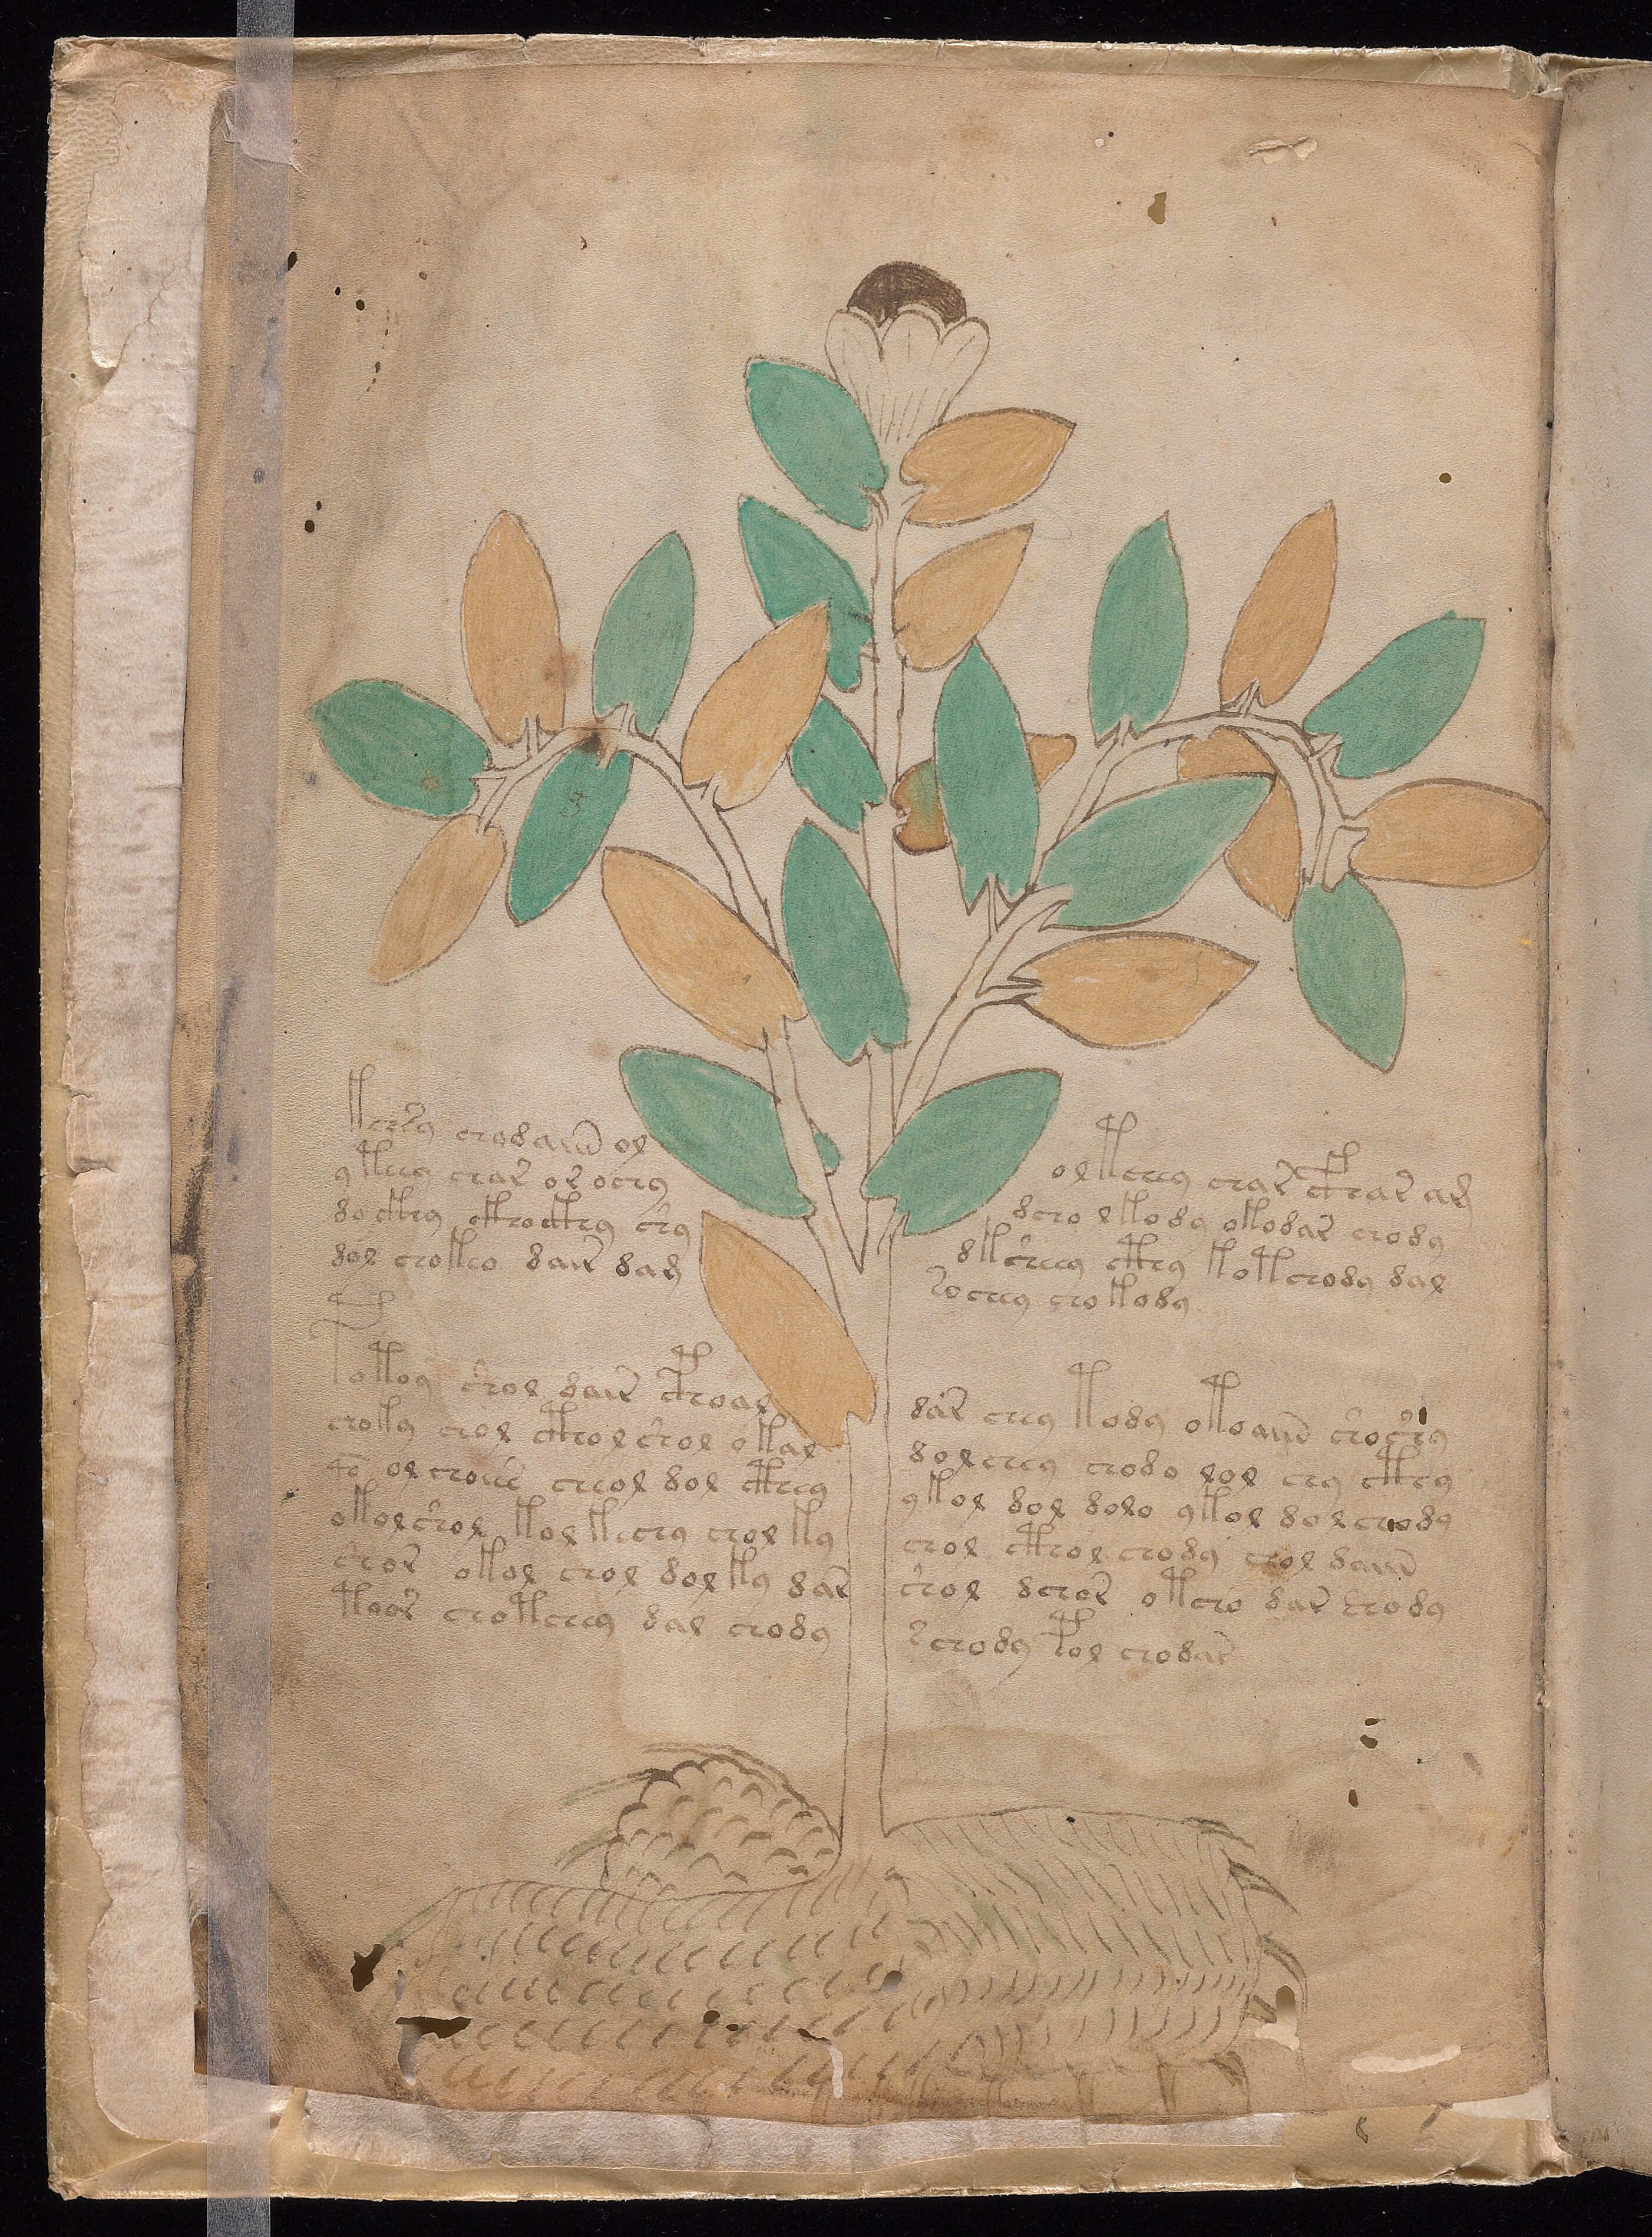
\includegraphics[width=0.25\textwidth]{f1v.jpg}
\end{wrapfigure}

\begin{locator}[P1, 1]\end{locator} {\eva kchsy chadaiin ol oltchey char cFhar am}\\
\begin{locator}[P1, 2]\end{locator} {\eva ytee\textcolor{orange}{y} char or ochy dcho lkody okodar chody}\\
\begin{locator}[P1, 3]\end{locator} {\eva do cKhy cKho cKhy Shy dkSheey cThy kotchody dal}\\
\begin{locator}[P1, 4]\end{locator} {\eva dol chokeo dair dam sochey chokody}\\

\vspace{1em}
\noindent\begin{locator}[P2, 5]\end{locator} {\eva potoy Shol dair cPhoal dar chey tody otoaiin ShoShy}\\
\begin{locator}[P2, 6]\end{locator} {\eva choky chol cThol Shol okal dolchey chodo lol chy cThy}\\
\begin{locator}[P2, 7]\end{locator} {\eva qo ol choee\textcolor{orange}{s} cheol dol cThey ykol dol dolo ykol do lchody}\\
\begin{locator}[P2, 8]\end{locator} {\eva okol\textcolor{orange}{$\frown$}Shol kol kechy chol ky chol cThol chody chol daiin}\\
\begin{locator}[P2, 9]\end{locator} {\eva Shor okol chol dol ky dar Shol dchor otcho dar Shody}\\
\begin{locator}[P2, 10]\end{locator} {\eva taor chotchey dal chody schody pol chodar}\\


%%%%%%
% 2R %
%%%%%%
\clearpage
\subsection{Folio 2, Recto}
\begin{wrapfigure}{r}{0.25\textwidth}
   \centering
   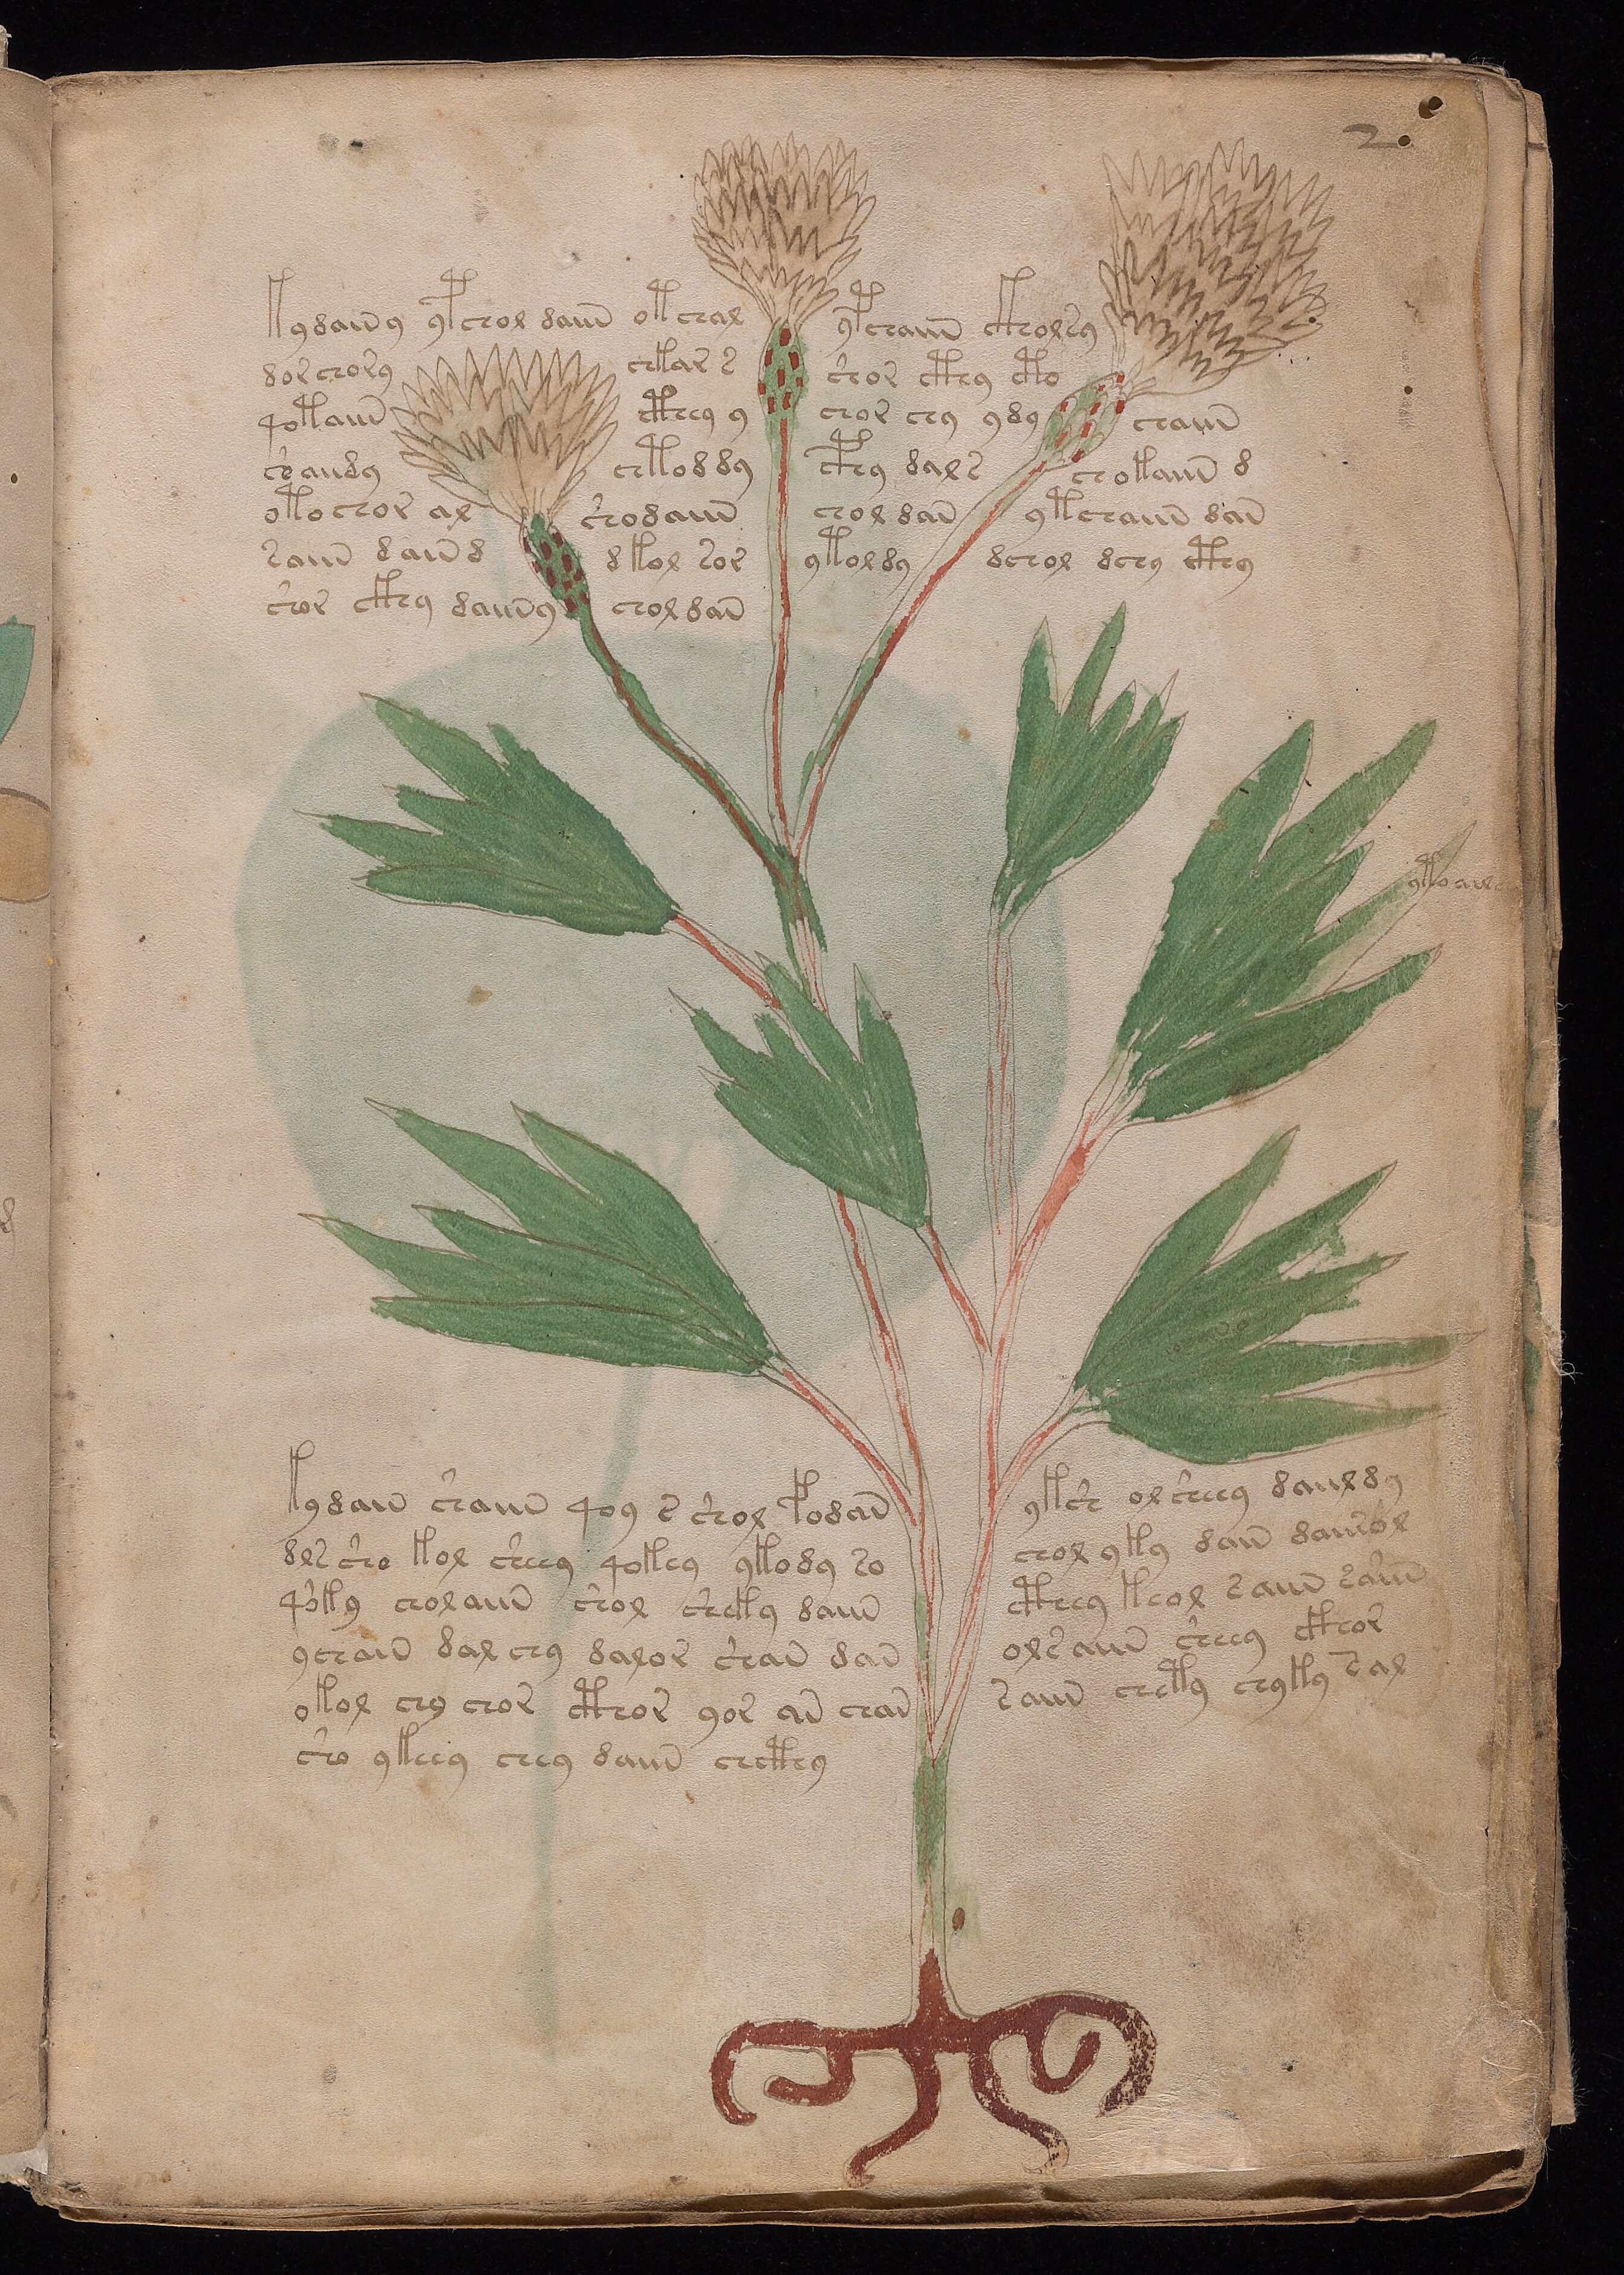
\includegraphics[width=0.25\textwidth]{f2r.jpg}
\end{wrapfigure}

\begin{locator}[P1, 1]\end{locator} {\eva kydainy ypchol daiin otchal ypchaiin cKholsy}\\
\begin{locator}[P1, 2]\end{locator} {\eva dorchory chkar s Shor cThy cTh}\\
\begin{locator}[P1, 3]\end{locator} {\eva qotaiin cThey y chor chy ydy chaiin}\\
\begin{locator}[P1, 4]\end{locator} {\eva chaindy chtod dy cPhy dals chokaiin d}\\
\begin{locator}[P1, 5]\end{locator} {\eva otochor al Shodaiin chol dan ytchaiin dan}\\
\begin{locator}[P1, 6]\end{locator} {\eva saiin daind dkol sor ytoldy dchol dchy cThy}\\
\begin{locator}[P1, 7]\end{locator} {\eva Shor cKhy daiiny chol dan}\\

\vspace{1em}
\noindent\begin{locator}[L1, 8]\end{locator} {\eva \textcolor{orange}{ytoaile*}}\\
\begin{locator}[L2, 9]\end{locator} {\eva \textcolor{orange}{***an}}\\

\vspace{1em}
\noindent\begin{locator}[P2, 10]\end{locator} {\eva kydain Shaiin qoy s Shol fodan ykSh olSheey daiildy}\\
\begin{locator}[P2, 11]\end{locator} {\eva dlsSho kol Sheey qokey ykody so chol yky dain daiirol}\\
\begin{locator}[P2, 12]\end{locator} {\eva qoky cholaiin Shol Sheky daiin cThey keol saiin saiin}\\
\begin{locator}[P2, 13]\end{locator} {\eva ychain dal chy dalor Shan dan olsaiin Sheey cKhor}\\
\begin{locator}[P2, 14]\end{locator} {\eva okol chy chor cThor yor an chan saiin chety chyky sal}\\
\begin{locator}[P2, 15]\end{locator} {\eva Sho ykeey chey daiin chcThy}\\


%%%%%%
% 2V %
%%%%%%
\clearpage
\subsection{Folio 2, Verso}
\begin{locator}[P1, 1]\end{locator} {\eva kooiin cheo pchor otaiin o dain chor dair Shty}\\
\begin{locator}[P1, 2]\end{locator} {\eva kcho kchy Sho Shol qotcho loeees qoty chor daiin}\\
\begin{locator}[P1, 3]\end{locator} {\eva otchy chor lShy chol chody chodain chcThy daiin}\\
\begin{locator}[P1, 4]\end{locator} {\eva Sho cholo cheor chodaiin}\\

\vspace{1em}
\noindent\begin{locator}[P2, 5]\end{locator} {\eva kchor Shy daiiin chcKhoy s Shey dor chol daiin}\\
\begin{locator}[P2, 6]\end{locator} {\eva dor chol chor chol keol chy chty daiin otchor chan}\\
\begin{locator}[P2, 7]\end{locator} {\eva daiin chotchey qoteeey chokeos chees chr cheaiin}\\
\begin{locator}[P2, 8]\end{locator} {\eva chokoiShe chor cheol chol dolody}\\


%%%%%%
% 3R %
%%%%%%
\clearpage
\subsection{Folio 3, Recto}
\begin{locator}[P1, 1]\end{locator} {\eva tSheos qopal chol cThol daimm}\\
\begin{locator}[P1, 2]\end{locator} {\eva ycheor chor dam qotcham cham}\\
\begin{locator}[P1, 3]\end{locator} {\eva ochor qocheor chol daiin cThy}\\
\begin{locator}[P1, 4]\end{locator} {\eva schey chor chal cham cham cho}\\
\begin{locator}[P1, 5]\end{locator} {\eva qokol chololy s cham cThol}\\
\begin{locator}[P1, 6]\end{locator} {\eva ychtaiin chor cThom otal\textcolor{orange}{$\frown$}dam}\\
\begin{locator}[P1, 7]\end{locator} {\eva otchol qodaiin chom Shom damo}\\
\begin{locator}[P1, 8]\end{locator} {\eva ySheor chor chol oky damo}\\
\begin{locator}[P1, 9]\end{locator} {\eva Sho *or Sheoldam otchody ol}\\
\begin{locator}[P1, 10]\end{locator} {\eva ydas chol cThom}\\

\vspace{1em}
\noindent\begin{locator}[P2, 11]\end{locator} {\eva pcheol Shol sols Sheol Shey}\\
\begin{locator}[P2, 12]\end{locator} {\eva okadaiin qokchor qoschodam ocThy}\\
\begin{locator}[P2, 13]\end{locator} {\eva qokeey qot Shey qokody qok\textcolor{orange}{Sh}ey cheody}\\
\begin{locator}[P2, 14]\end{locator} {\eva chor qodair okeey qokeey}\\

\vspace{1em}
\noindent\begin{locator}[P3, 15]\end{locator} {\eva tSheoarom Shor or chor olchsy chom otchom oporar}\\
\begin{locator}[P3, 16]\end{locator} {\eva oteol chol s cheol ekShy qokeom qokol daiin soleeg}\\
\begin{locator}[P3, 17]\end{locator} {\eva soeom okeom yteody qokeeo\textcolor{orange}{$\frown$}dal sam}\\

\vspace{1em}
\noindent\begin{locator}[P4, 18]\end{locator} {\eva pcheoldom Shodaiin qopchor qopol opchol qoty otolom}\\
\begin{locator}[P4, 19]\end{locator} {\eva otchor ol cheor qoeor dair qoteol qosaiin chor cThy}\\
\begin{locator}[P4, 20]\end{locator} {\eva ycheor chol odaiin chol s aiin okolor am}\\


%%%%%%
% 3V %
%%%%%%
\clearpage
\subsection{Folio 3, Verso}
\begin{locator}[P1, 1]\end{locator} {\eva koaiin cPhor qotoy Sha cKhol ykoaiin s oly}\\
\begin{locator}[P1, 2]\end{locator} {\eva daiidy qot\textcolor{orange}{ch}ol okchor okor olytol dol dar}\\
\begin{locator}[P1, 3]\end{locator} {\eva okom chol Shol seees chom cheeykam okai}\\
\begin{locator}[P1, 4]\end{locator} {\eva qodar \textcolor{orange}{ch}s \textcolor{orange}{ch}y kcheol okal do\textcolor{orange}{$\frown$}r chear een}\\
\begin{locator}[P1, 5]\end{locator} {\eva y\textcolor{orange}{ch}ear otchal \textcolor{orange}{ch}or \textcolor{orange}{ch}ar cKhy}\\
\begin{locator}[P1, 6]\end{locator} {\eva or cheor kor chodaly chom}\\

\vspace{1em}
\noindent\begin{locator}[P2, 7]\end{locator} {\eva tchor otcham chor cFham s}\\
\begin{locator}[P2, 8]\end{locator} {\eva ykchy kchom chor ch\textcolor{orange}{cKh}ol oka}\\
\begin{locator}[P2, 9]\end{locator} {\eva ytcheear okeol cThodoaly chor cThy}\\
\begin{locator}[P2, 10]\end{locator} {\eva ochor daiin qokShol daiim chol okary}\\
\begin{locator}[P2, 11]\end{locator} {\eva Sho ShocKho cKhy tchor chodaiin chom}\\
\begin{locator}[P2, 12]\end{locator} {\eva oSh chodair ytchy tchor kcham s}\\
\begin{locator}[P2, 13]\end{locator} {\eva Shar Shkaiin qokchy yty cThal chky}\\
\begin{locator}[P2, 14]\end{locator} {\eva dain Sheam yteam}\\


%%%%%%
% 4R %
%%%%%%
\clearpage
\subsection{Folio 4, Recto}
\begin{locator}[P1, 1]\end{locator} {\eva kodalchy chpady Sheol ol Sheey qotey doiin chor ytoy}\\
\begin{locator}[P1, 2]\end{locator} {\eva dchor chol Shol cThol Shtchy chaiin \textcolor{orange}{*}s choraiin chom}\\
\begin{locator}[P1, 3]\end{locator} {\eva otchol chol chy chaiin qotaiin daiin Shain}\\
\begin{locator}[P1, 4]\end{locator} {\eva qotchol chy yty daiin okaiin cThy}\\

\vspace{1em}
\noindent\begin{locator}[P2, 5]\end{locator} {\eva pydaiin qotchy dy tydy}\\
\begin{locator}[P2, 6]\end{locator} {\eva chor Shytchy dy tche\textcolor{orange}{e}y}\\
\begin{locator}[P2, 7]\end{locator} {\eva qotaiin cThol daiin cThom}\\
\begin{locator}[P2, 8]\end{locator} {\eva Shor Shol Shol cThy cPholdy}\\
\begin{locator}[P2, 9]\end{locator} {\eva daiin cKhochy tchy koraiin}\\
\begin{locator}[P2, 10]\end{locator} {\eva odal Shor ShyShol cPhaiin}\\
\begin{locator}[P2, 11]\end{locator} {\eva qotchoiin Sheyr qoty}\\
\begin{locator}[P2, 12]\end{locator} {\eva soiin chaiin chaiin}\\
\begin{locator}[P2, 13]\end{locator} {\eva daiin cThey}\\


%%%%%%
% 4V %
%%%%%%
\clearpage
\subsection{Folio 4, Verso}
\begin{locator}[P1, 1]\end{locator} {\eva pchooiin kSheo kchoy chopchy dolds dlod}\\
\begin{locator}[P1, 2]\end{locator} {\eva ol chey chy cThy Shkchor Sheo cheory choldy}\\
\begin{locator}[P1, 3]\end{locator} {\eva Sho Sho chaiin Shaiin daiin qodaiin o ar am}\\
\begin{locator}[P1, 4]\end{locator} {\eva qokShy qocThy choteol daiin cThey choaiin}\\
\begin{locator}[P1, 5]\end{locator} {\eva Shor Sheey cto otoiin Shey qotchoiin chodain}\\
\begin{locator}[P1, 6]\end{locator} {\eva ytchoy Shokchy cPhody}\\

\vspace{1em}
\noindent\begin{locator}[P2, 7]\end{locator} {\eva torchy Sheeor chor Shokchy cPhydy}\\
\begin{locator}[P2, 8]\end{locator} {\eva olaen chor cThol Sho otor cThory}\\
\begin{locator}[P2, 9]\end{locator} {\eva qooko iiincheom chcThy Shoky daiin}\\
\begin{locator}[P2, 10]\end{locator} {\eva otaiin Sheo okeody chol chokeody}\\
\begin{locator}[P2, 11]\end{locator} {\eva Sho kcheor Shody Shtaiin qotol daiin}\\
\begin{locator}[P2, 12]\end{locator} {\eva qokoy Sho okeol s keey Shar char ody}\\
\begin{locator}[P2, 13]\end{locator} {\eva Shody s cheor chokody Shodaiin qoty}\\
\begin{locator}[P2, 14]\end{locator} {\eva ochody chykey chtody}\\


%%%%%%
% 5R %
%%%%%%
\clearpage
\subsection{Folio 5, Recto}
\begin{locator}[P1, 1]\end{locator} {\eva kShody fchoy chkoy oaiin oar olsy chody dkShy dy}\\
\begin{locator}[P1, 2]\end{locator} {\eva ochey okey qokaiin Sho cKhoy cThey chey oka*or otol}\\
\begin{locator}[P1, 3]\end{locator} {\eva qoaiin otan chy daiin oteeen cho cThy otchy qotcho dy}\\
\begin{locator}[P1, 4]\end{locator} {\eva otain Sheody chan s cheor chocThy}\\

\vspace{1em}
\noindent\begin{locator}[P2, 5]\end{locator} {\eva tShy Shody qoaiin cholols Sho qotcheo daiin Shodaiin}\\
\begin{locator}[P2, 6]\end{locator} {\eva Sho cheor chey qoeeey qoykeeey qoeor cThy ShotShy dy}\\
\begin{locator}[P2, 7]\end{locator} {\eva qotoeey keey cheo kchy Shody}\\


%%%%%%
% 5V %
%%%%%%
\clearpage
\subsection{Folio 5, Verso}
\begin{locator}[P1, 1]\end{locator} {\eva kocheor chor ytchey pShod chols chodaiin ytoiiin daiin}\\
\begin{locator}[P1, 2]\end{locator} {\eva dchol \textcolor{orange}{S}y chol otaiin dain cThor chots ychopordg}\\
\begin{locator}[P1, 3]\end{locator} {\eva qotcho ytor daiin daiin otchor daii\textcolor{orange}{n} qo darchor do}\\
\begin{locator}[P1, 4]\end{locator} {\eva qotor Shees otol ykoiin Shol daiin cThor okchy taiin}\\
\begin{locator}[P1, 5]\end{locator} {\eva Shokeeol chor cheotol otchol daiin dal chol chotaiin}\\
\begin{locator}[P1, 6]\end{locator} {\eva otol chol dairodg}\\


%%%%%%
% 6R %
%%%%%%
\clearpage
\subsection{Folio 6, Recto}
\begin{locator}[P1, 1]\end{locator} {\eva foar y Shol cholor cPhol chor chcKh chopchol otcham}\\
\begin{locator}[P1, 2]\end{locator} {\eva daiin chcKhy chor chor kar cThy cThor chotols}\\
\begin{locator}[P1, 3]\end{locator} {\eva poeear kShor choky os cheoee\textcolor{orange}{e}s ykeor ytaiin dar}\\
\begin{locator}[P1, 4]\end{locator} {\eva dar cho s Sheor chocThy otcham yaiir chy}\\
\begin{locator}[P1, 5]\end{locator} {\eva tar okoiin Shees ytaly cThaiin odam}\\
\begin{locator}[P1, 6]\end{locator} {\eva or al daiin cKham okom cThaiin ydaiin}\\
\begin{locator}[P1, 7]\end{locator} {\eva daiin qodaiin cho s chol okaiin s}\\
\begin{locator}[P1, 8]\end{locator} {\eva ychol cKhor pchar Sheo cKhaiin}\\
\begin{locator}[P1, 9]\end{locator} {\eva dar Sh\textcolor{orange}{e}ol skaiiodar otaiin chory}\\
\begin{locator}[P1, 10]\end{locator} {\eva tchor cTheod chy Shor odShe od}\\
\begin{locator}[P1, 11]\end{locator} {\eva ychar olchad ol chokaiin}\\
\begin{locator}[P1, 12]\end{locator} {\eva or Shol cThom chor cThy}\\
\begin{locator}[P1, 13]\end{locator} {\eva qocThol \textcolor{orange}{y}odaiin cThy}\\
\begin{locator}[P1, 14]\end{locator} {\eva ySho taiin y kaiim}\\


%%%%%%
% 6V %
%%%%%%
\clearpage
\subsection{Folio 6, Verso}
\begin{locator}[P1, 1]\end{locator} {\eva koar y sar \textcolor{orange}{c}heekar qoar Shor chapchy s chear char otchy}\\
\begin{locator}[P1, 2]\end{locator} {\eva oees chor chcKhy qoekchar cheas odaii\textcolor{orange}{i}n kchey chor chaiin}\\
\begin{locator}[P1, 3]\end{locator} {\eva qoair cKhy chol oochocKhy chekchoy cKhy okol rychos}\\
\begin{locator}[P1, 4]\end{locator} {\eva y ShcKhy ytchoy sos y\textcolor{orange}{$\frown$}dady dchy dey okody ytody}\\
\begin{locator}[P1, 5]\end{locator} {\eva dair \textcolor{orange}{Sha} chodam dam okor oty doldom}\\

\vspace{1em}
\noindent\begin{locator}[P2, 6]\end{locator} {\eva tchody ShocThol chocThey s}\\
\begin{locator}[P2, 7]\end{locator} {\eva ychos ychol daiin cThol dol}\\
\begin{locator}[P2, 8]\end{locator} {\eva ychor chor okchey qokom}\\
\begin{locator}[P2, 9]\end{locator} {\eva oeeo dal chor cThom s}\\
\begin{locator}[P2, 10]\end{locator} {\eva qokch\textcolor{orange}{od} ychear kchdy}\\
\begin{locator}[P2, 11]\end{locator} {\eva lor char otam cThom dy}\\
\begin{locator}[P2, 12]\end{locator} {\eva ytchos Shy qokam cThy}\\
\begin{locator}[P2, 13]\end{locator} {\eva yodaiin cThy s chor oees or}\\
\begin{locator}[P2, 14]\end{locator} {\eva qokor chol cThol tchalody}\\
\begin{locator}[P2, 15]\end{locator} {\eva chocKhy s os chy sain or}\\
\begin{locator}[P2, 16]\end{locator} {\eva ochy cThar cThar cThy}\\
\begin{locator}[P2, 17]\end{locator} {\eva y chaiir cKhal cThodam dy}\\
\begin{locator}[P2, 18]\end{locator} {\eva ytcho\textcolor{orange}{$\frown$}cThol ches cThor}\\
\begin{locator}[P2, 19]\end{locator} {\eva ocholy kchos chy dor}\\
\begin{locator}[P2, 20]\end{locator} {\eva dchor choldar okol daiin}\\
\begin{locator}[P2, 21]\end{locator} {\eva ycheor chor ocTham}\\


%%%%%%
% 7R %
%%%%%%
\clearpage
\subsection{Folio 7, Recto}
\begin{locator}[P1, 1]\end{locator} {\eva fchodaiin Shopchey qko Shey qoos Sheey ch\textcolor{orange}{a}rochy}\\
\begin{locator}[P1, 2]\end{locator} {\eva dcheey keor Shor dold dchey kchey otchy cheody}\\
\begin{locator}[P1, 3]\end{locator} {\eva oeeees cheodaiin Sheey ytcheey qotchy chald}\\
\begin{locator}[P1, 4]\end{locator} {\eva qokcho cho lochey daiin ychey kchos odaiin}\\
\begin{locator}[P1, 5]\end{locator} {\eva oaiir otaiin}\\

\vspace{1em}
\noindent\begin{locator}[P2, 6]\end{locator} {\eva kSholo\textcolor{orange}{Sh}ey qotoees chkoldy otchor choaiin}\\
\begin{locator}[P2, 7]\end{locator} {\eva dShoy cThol chol otchol dain Shody Shol chotchy}\\
\begin{locator}[P2, 8]\end{locator} {\eva okchey deeeese choty qokchy Shol keey choty dain}\\
\begin{locator}[P2, 9]\end{locator} {\eva qokechy olchoiin chol cPhey ShcKhy chochy kchod}\\
\begin{locator}[P2, 10]\end{locator} {\eva schain chor daiin chcKhy}\\


%%%%%%
% 7V %
%%%%%%
\clearpage
\subsection{Folio 7, Verso}
\begin{locator}[P1, 1]\end{locator} {\eva polyShy Shey tchody qopchy otShol dy\textcolor{orange}{$\frown$}daiin tShodody}\\
\begin{locator}[P1, 2]\end{locator} {\eva chochy cThy daiin qoky chcPhhy daiin cThol cThy cThd}\\
\begin{locator}[P1, 3]\end{locator} {\eva qokchy dykchy chkeey kShy ky ty dor cheey ol\textcolor{orange}{$\frown$}cheol\textcolor{orange}{$\frown$}dy}\\
\begin{locator}[P1, 4]\end{locator} {\eva choteeen oeear choschy dain Sho\textcolor{orange}{$\frown$}kShy Shol deees\textcolor{orange}{$\frown$}dol}\\
\begin{locator}[P1, 5]\end{locator} {\eva dchodaiin qotchy cheey tcheey}\\

\vspace{1em}
\noindent\begin{locator}[P2, 6]\end{locator} {\eva kchor Sheod Sheodaiin Shodaiin okSho\textcolor{orange}{$\frown$}lShol dai\textcolor{orange}{r} qos}\\
\begin{locator}[P2, 7]\end{locator} {\eva okSho\textcolor{orange}{$\frown$}deeen chor\textcolor{orange}{$\frown$}cheor odaiin Shotch\textcolor{orange}{*} dol dol dor aiin}\\
\begin{locator}[P2, 8]\end{locator} {\eva qoteeeo rcho\textcolor{orange}{$\frown$}cheeody qotchey tey okchor daiin}\\
\begin{locator}[P2, 9]\end{locator} {\eva Sho keeo daiir chokchy dor deol dy dol daiin}\\


%%%%%%
% 8R %
%%%%%%
\clearpage
\subsection{Folio 8, Recto}
\begin{locator}[P1, 1]\end{locator} {\eva pShol chor otShal chopy cPhol chody Shy cFhodar Shor}\\
\begin{locator}[P1, 2]\end{locator} {\eva tchty Sh kcheals Sho okche do dchy dain al}\\
\begin{locator}[P1, 3]\end{locator} {\eva chodar Shy ry chodaiin Shokchy chor dy}\\
\begin{locator}[P1, 4]\end{locator} {\eva qotor chor chor Sheey dchol Shesed chofchy dam}\\
\begin{locator}[P1, 5]\end{locator} {\eva okchey do r cheeey dy ky scho chky ckooaiin ch\textcolor{orange}{o} taiin}\\
\begin{locator}[P1, 6]\end{locator} {\eva toSh ckcheey koltoldy Shy cho\textcolor{orange}{e}ty cheeody sol}\\
\begin{locator}[P1, 7]\end{locator} {\eva choto kchoan choor dain}\\
\begin{locator}[T1, 8]\end{locator} {\eva \textcolor{orange}{d}cho daiin}\\

\vspace{1em}
\noindent\begin{locator}[P2, 1]\end{locator} {\eva tchoep Sho pcheey pchey ofchey dSheey Shol\textcolor{orange}{$\frown$}daiin Shor}\\
\begin{locator}[P2, 9]\end{locator} {\eva daiin cheey teeodan dy cheocThy okSheo dol dair\textcolor{orange}{g}}\\
\begin{locator}[P2, 10]\end{locator} {\eva Shol cheodaiin daiin do ytchody chot choty otariin}\\
\begin{locator}[P2, 11]\end{locator} {\eva qochodaiin Shotokody chotol}\\
\begin{locator}[T2, 12]\end{locator} {\eva okokchod\textcolor{orange}{g}}\\

\vspace{1em}
\noindent\begin{locator}[P3, 13]\end{locator} {\eva cTho cThey Shol chofydy Sho chey kShey lody cholal}\\
\begin{locator}[P3, 14]\end{locator} {\eva dchey cKhol chol chey kchs chy \textcolor{orange}{cT}odaiin dol daiiirchy cKhy}\\
\begin{locator}[P3, 15]\end{locator} {\eva ychey kchokchy chsey kchy scheaiin cThaichar cThy dar}\\
\begin{locator}[P3, 16]\end{locator} {\eva chol dchy qokar chl aiin chean c\textcolor{orange}{K}y char chaiin}\\
\begin{locator}[P3, 17]\end{locator} {\eva okar cPhaiin chaiin el daiin chor cha rchealcham}\\
\begin{locator}[P3, 18]\end{locator} {\eva sair cheain cPhol dar Shol kaiin Shol kaiin daikam}\\
\begin{locator}[P3, 19]\end{locator} {\eva or chokesey Shey okal chal}\\
\begin{locator}[T3, 20]\end{locator} {\eva schol sair}\\


%%%%%%
% 8V %
%%%%%%
\clearpage
\subsection{Folio 8, Verso}
\begin{locator}[P1, 1]\end{locator} {\eva cThod soocTh sol Shol otol chol opcheaiin opydaiin saiin}\\
\begin{locator}[P1, 2]\end{locator} {\eva ShcThal sar chor Sheaiin Shor chykchy otaiin cty}\\
\begin{locator}[P1, 3]\end{locator} {\eva qody cheal sy chory chear Shol chaiin Shaiin dolar}\\
\begin{locator}[P1, 4]\end{locator} {\eva dShol Shol d\textcolor{orange}{a}l chean cThar Shealy daiin chary}\\
\begin{locator}[P1, 5]\end{locator} {\eva chol chol dar otchar etaiin cThol dar}\\
\begin{locator}[P1, 6]\end{locator} {\eva daiin cThan ytchy chey kaiin dain ar}\\
\begin{locator}[P1, 7]\end{locator} {\eva Sho kchol dar Shey cThar chotain ry}\\
\begin{locator}[P1, 8]\end{locator} {\eva okchol kSh chol chol chol cThaiin dain}\\
\begin{locator}[P1, 9]\end{locator} {\eva Shol orchl chokchy chol cThor chaiin}\\
\begin{locator}[P1, 10]\end{locator} {\eva scharchy oeesody kchey pchy cPharom}\\
\begin{locator}[P1, 11]\end{locator} {\eva sorain}\\

\vspace{1em}
\noindent\begin{locator}[P2, 12]\end{locator} {\eva pchar cho rol dal Shear ch\textcolor{orange}{ch}otaiin chal daiin}\\
\begin{locator}[P2, 13]\end{locator} {\eva kchor otchar oky chokain keoky otorchy satar}\\
\begin{locator}[P2, 14]\end{locator} {\eva Shor okol lokaiin Shol kol char cThey tchy cKham}\\
\begin{locator}[P2, 15]\end{locator} {\eva or chol cheen chcky chor cheain char cheeky chor ry}\\
\begin{locator}[P2, 16]\end{locator} {\eva chor chear chear oteey dchor chodey cho raiin}\\
\begin{locator}[P2, 17]\end{locator} {\eva dain chear daiin}\\


%%%%%%
% 9R %
%%%%%%
\clearpage
\subsection{Folio 9, Recto}

\begin{locator}[P1, 1]\end{locator} {\eva tydlo choly cThor orchey s Shy odaiin sary Shor cThy}\\
\begin{locator}[P1, 2]\end{locator} {\eva oykeey chol ytaiin okchody toeoky okoiin dy or chaiin}\\
\begin{locator}[P1, 3]\end{locator} {\eva toiin cPhy qotod otaiin cThy okor chey cThod ram}\\
\begin{locator}[P1, 4]\end{locator} {\eva yShy chokcho chcThod Shor Shaiin otar dor ytol dayty}\\
\begin{locator}[P1, 5]\end{locator} {\eva daiin chor sor cThy chokoiin Shol dSholdy otchol ot dy}\\

\vspace{1em}
\noindent\begin{locator}[P2, 6]\end{locator} {\eva pShoain cThyaiin okaiir cFhodoral Shar sy Shydal chdy}\\
\begin{locator}[P2, 7]\end{locator} {\eva or chol chytchy tchol ytor qotol chyky chodar aiin}\\
\begin{locator}[P2, 8]\end{locator} {\eva qotcho qokchy cThey koraiin okain d dal s olSho cThy}\\
\begin{locator}[P2, 9]\end{locator} {\eva ocho cThy choc\textcolor{orange}{T}oy chodykchy saiin dchy daiin}\\
\begin{locator}[T1, 10]\end{locator} {\eva ytchas oraiin chk\textcolor{orange}{o}r}\\


%%%%%%
% 9V %
%%%%%%
\clearpage
\subsection{Folio 9, Verso}


%%%%%%%%%%%%%%
% REFERENCES %
%%%%%%%%%%%%%%
\clearpage
\printbibliography

\end{document}